	%!TEX root = ../../Main.tex
\graphicspath{{Chapters/Userinterface/}}
%-------------------------------------------------------------------------------


\section{Brugergrænseflade}
I dette afsnit gives der et overblik over brugergrænsefladen og brugerens mulighed for interaktion med denne. Afsnittet er bygget op af billeder, hvor hvert billede viser brugergrænsefladens visuelle struktur. \\

Første display man møder er "Welcome". Her går systemet igang med at initialisere de forskellige moduler og drivere, således de er klar til brug.
\begin{figure}[H]
	\centering
	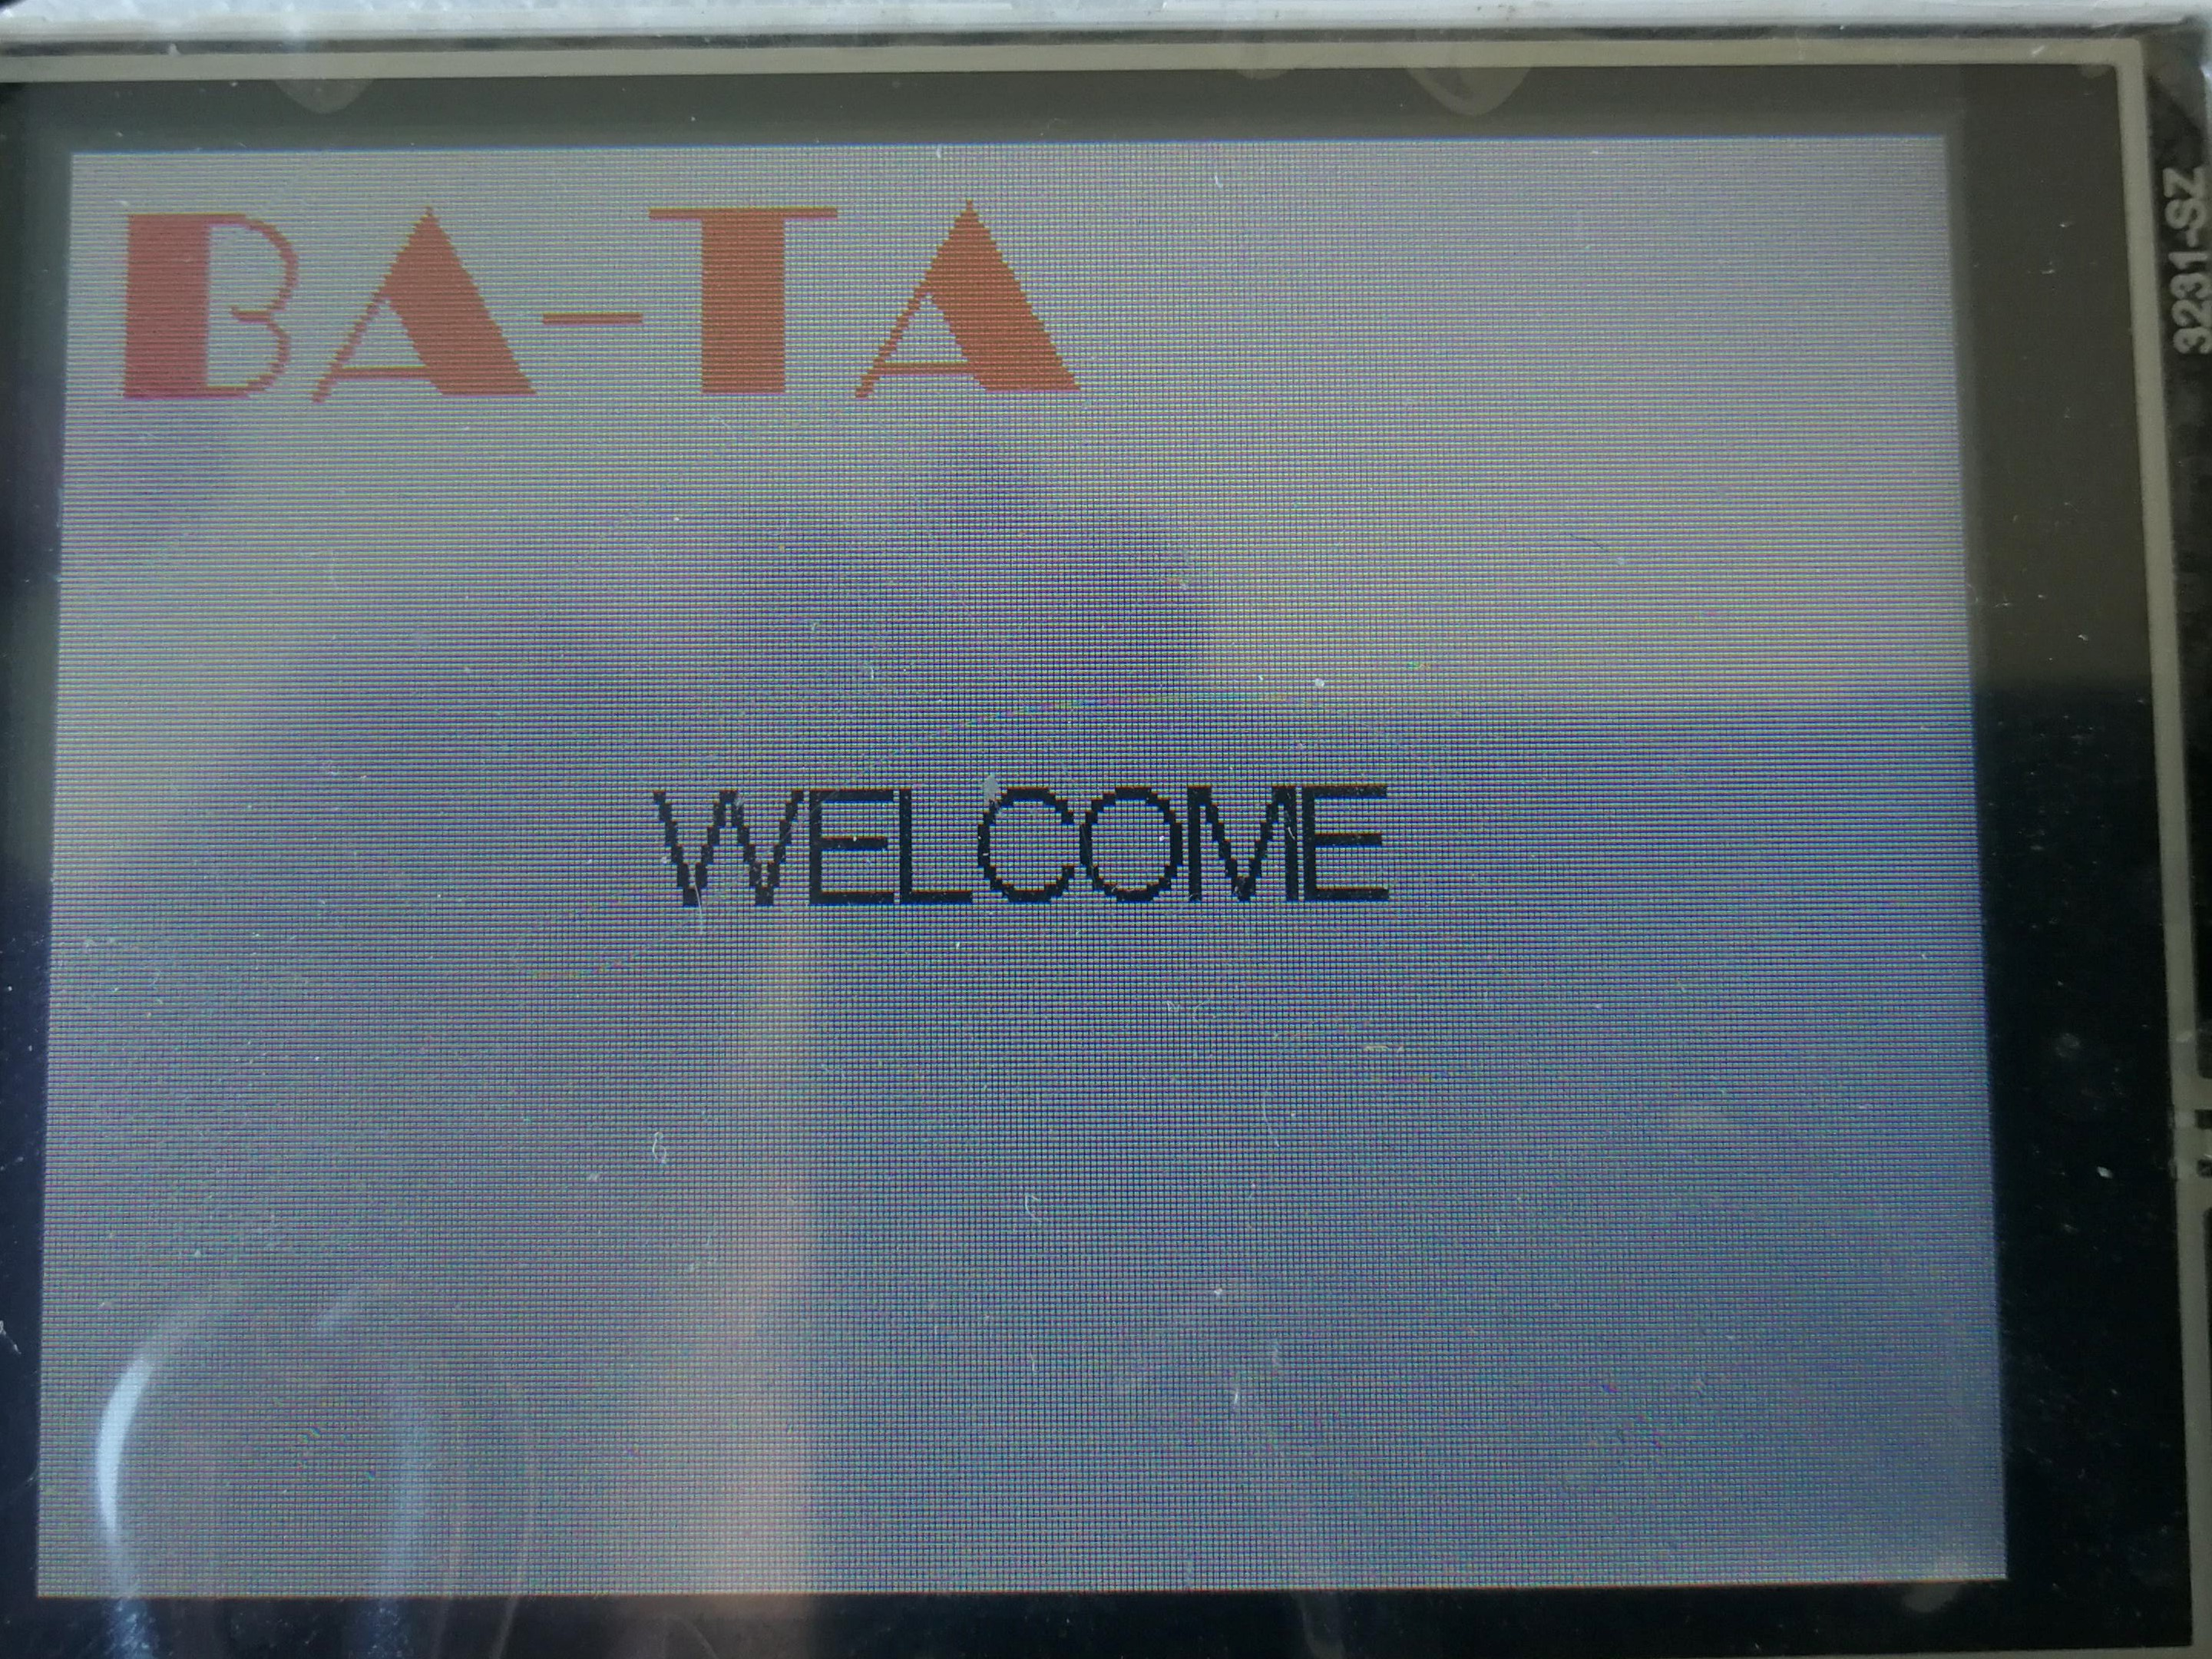
\includegraphics[width = 300 pt]{Img/welcome.jpg}
	\caption{Welcome}
	\label{fig:welcome}
\end{figure}



Næste display er hovedmenuen for systemet, hvor der er tre forskellige muligheder, som ses på figur     \ref{fig:start}. Yderligere ses der 4 trykknapper, hvor brugeren kan interagere med systemet.

\begin{itemize}  
	\item  Med "Enter" vælger brugeren en funktion
	\item "Back" gør brugeren i stand til at gå tilbage til hovedmenuen, hvis man forinden har trykket "ENTER" ved "ADD DEVICE" eller "REMOVE DEVICE".
	\item "Up" og "Down" flytter pilen, hhv. op og ned.
\end{itemize}

 Herudover ses der en farvet boks øverst i højre hjørne, som indikerer låsens tilstand. Denne lås viser grøn ved låst op og rød ved låst. Øverst til venstre på skærmen vises systemets logo.    
\begin{figure}[H]
	\centering
	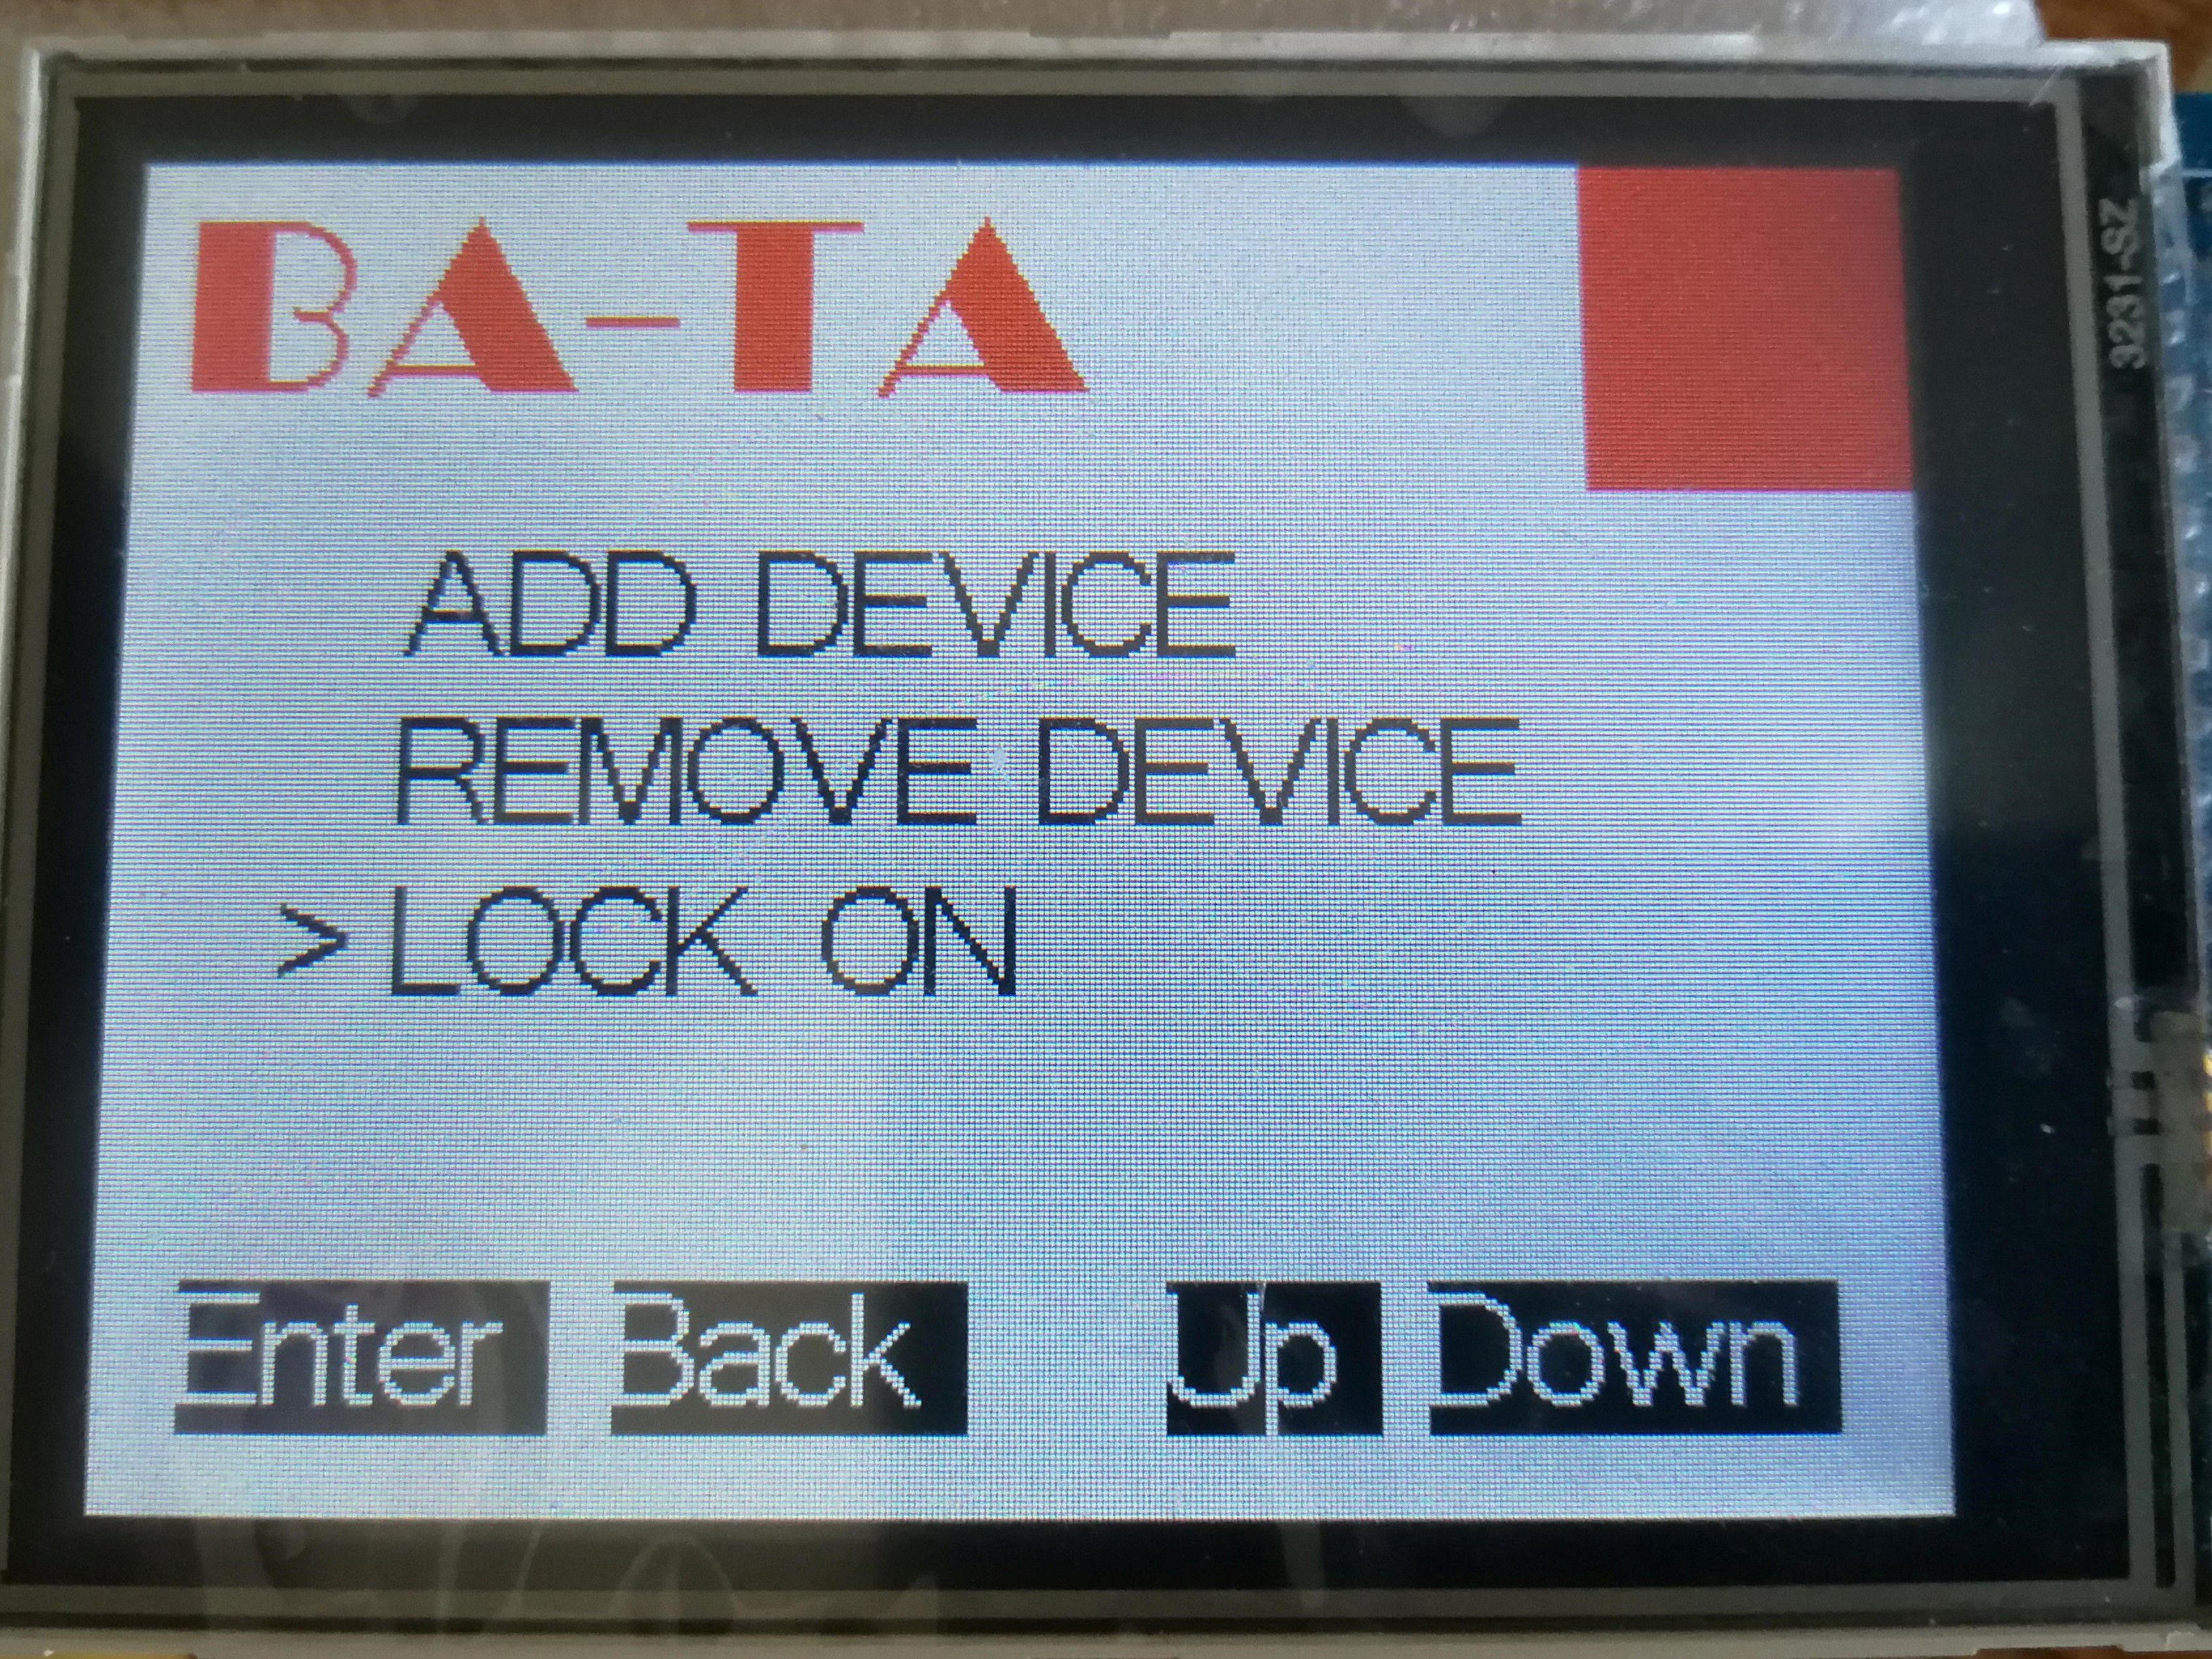
\includegraphics[width = 300 pt]{Img/start.jpg}
	\caption{Hovedmenu}
	\label{fig:start}
\end{figure}

Hvis brugeren trykker på "ADD DEVICE", søger BA-TA efter de 4 stærkeste Bluetooth signaler, som er indenfor rækkevidde. 
\begin{figure}[H]
	\centering
	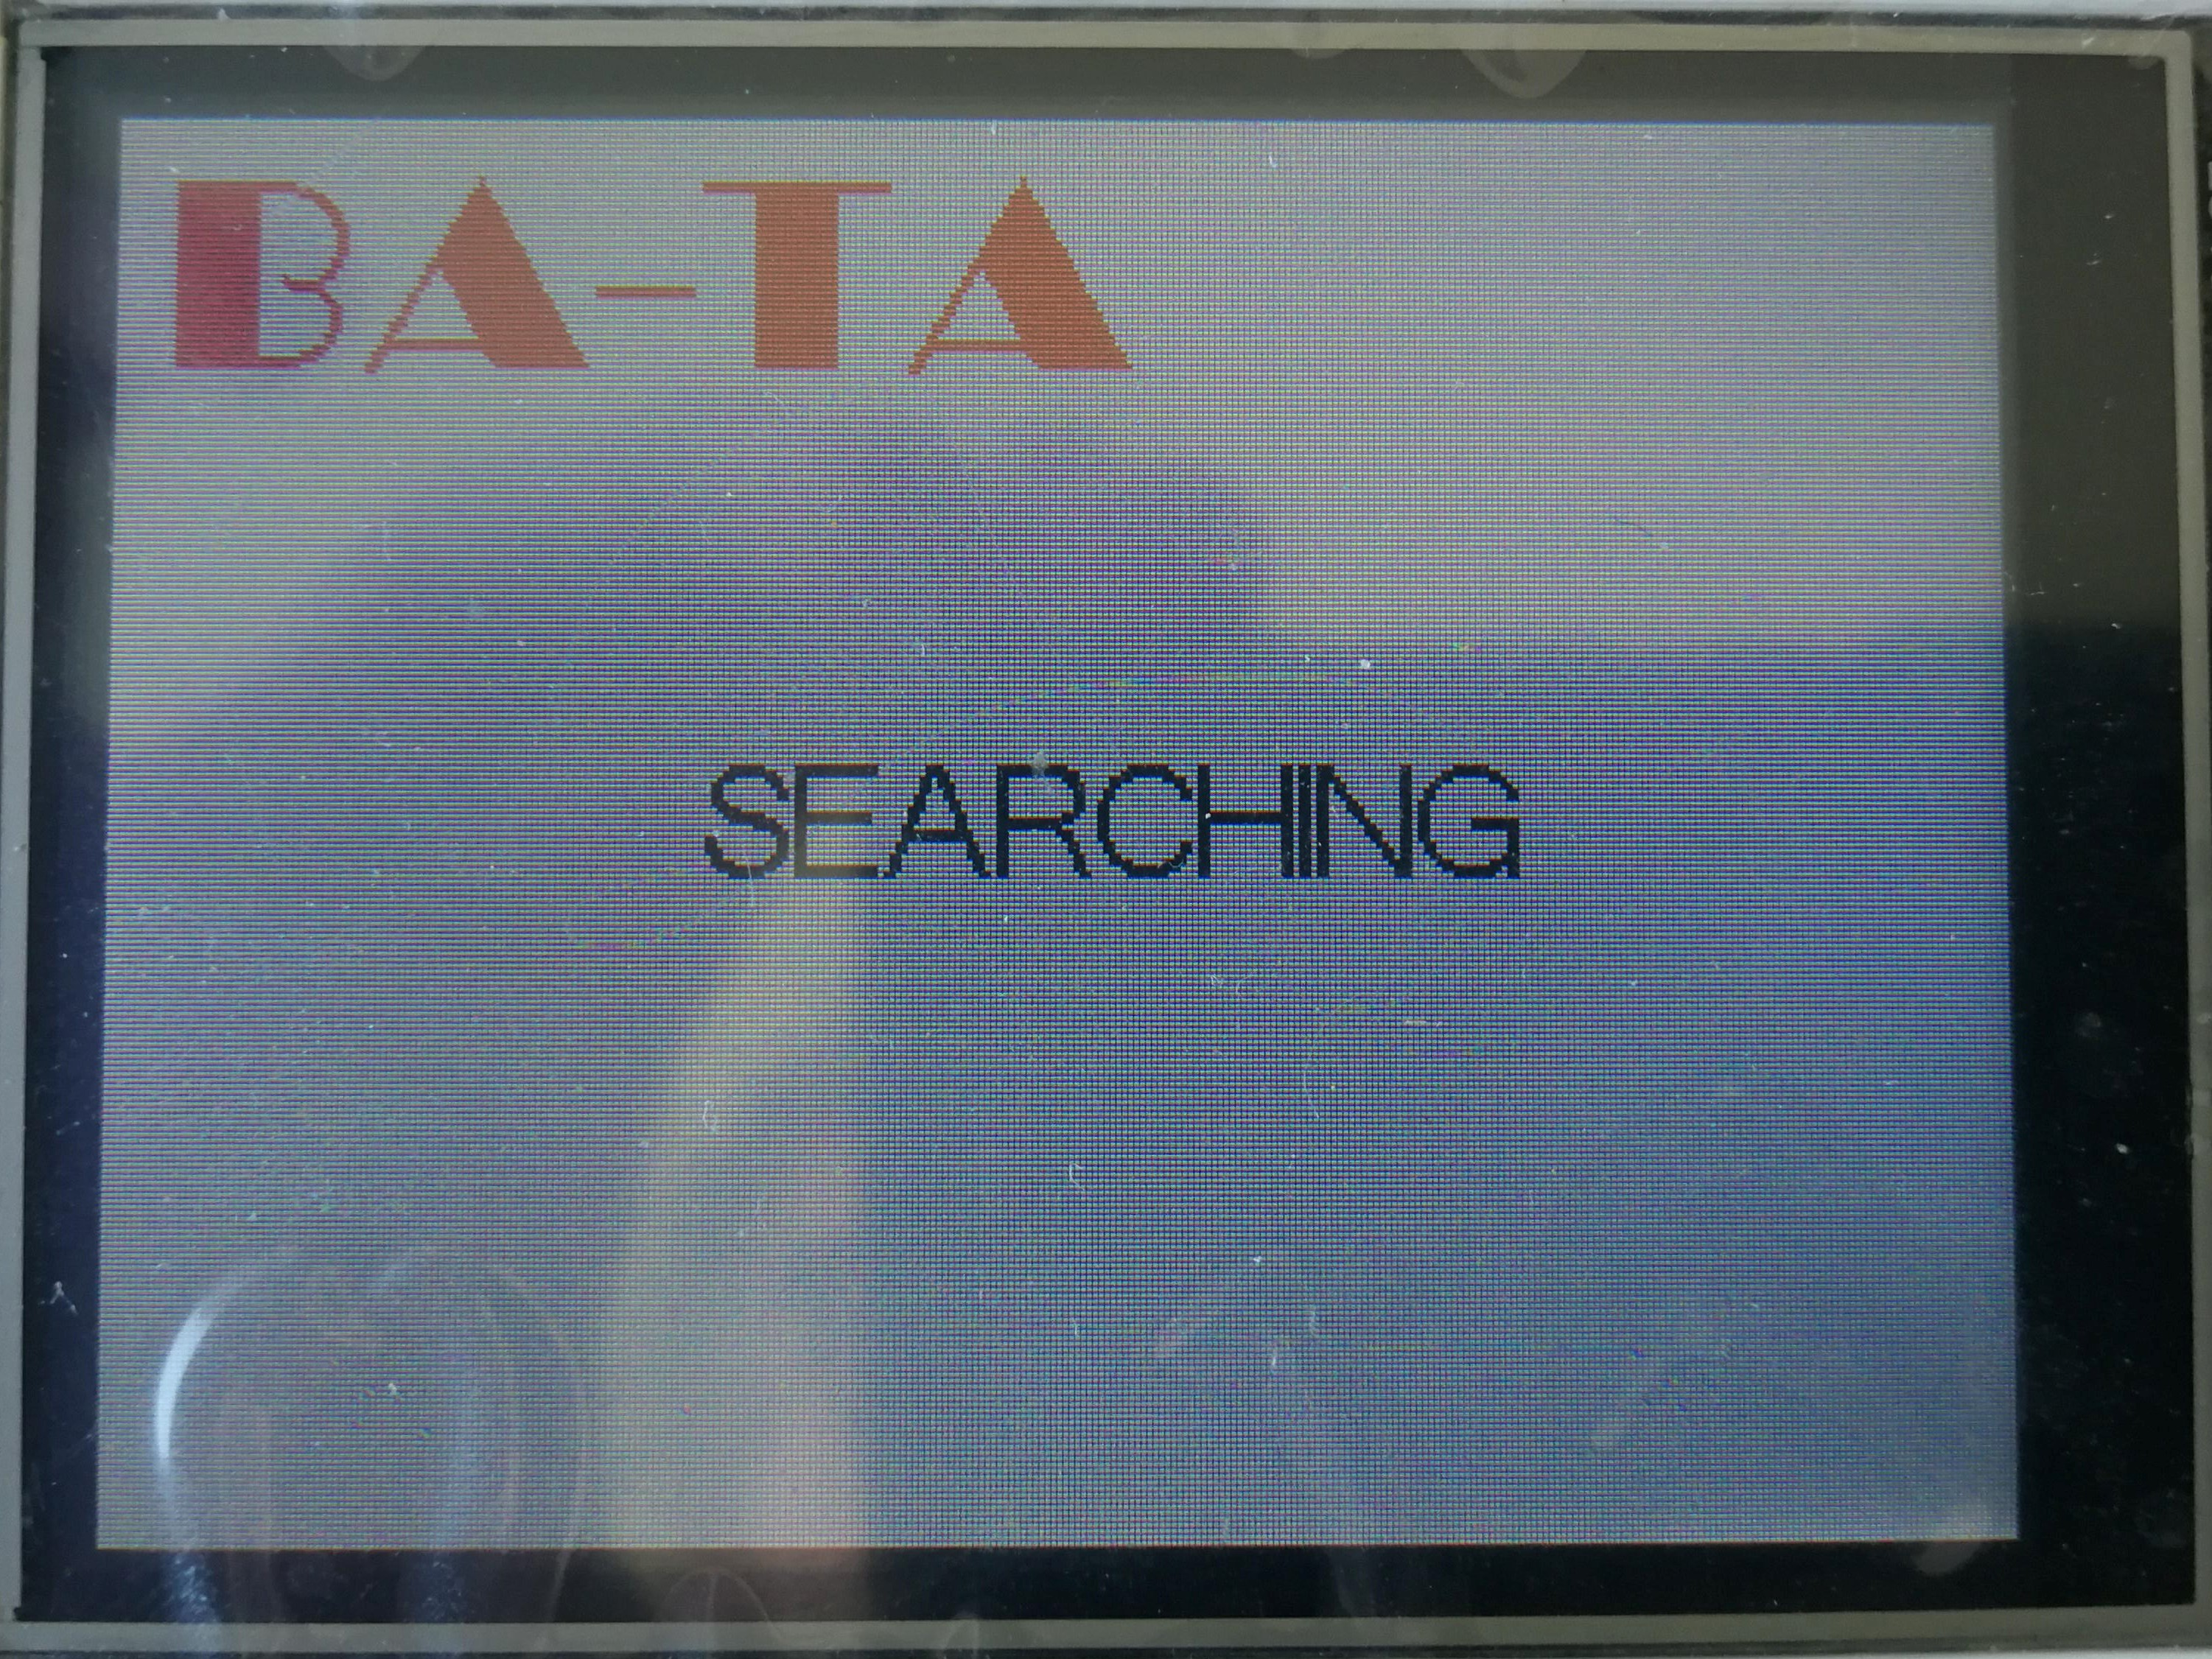
\includegraphics[width = 300 pt]{Img/Searching.jpg}
	\caption{Searching}
	\label{fig:Searching}
\end{figure}
Herefter vises de fundne Bluetooth-enheder, som systemets Bluetooth-modul har fundet. Dette ses på figur \ref{fig:devices}.
\begin{figure}[H]
	\centering
	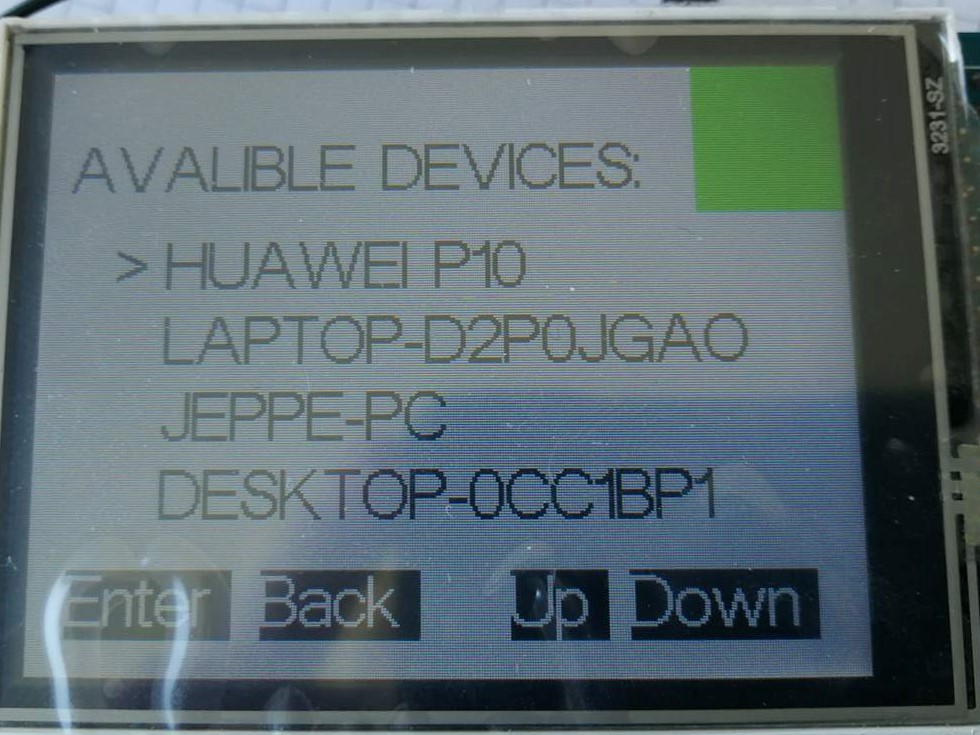
\includegraphics[width = 300 pt]{Img/devices.jpg}
	\caption{Tilgængelige enheder}
	\label{fig:devices}
\end{figure}
Hvis der vælges en enhed ved et tryk på "Enter", så vises navnet på den valgte enhed. Herefter går skærmens tilstand tilbage til hovedmenuen. 
\begin{figure}[H]
	\centering
	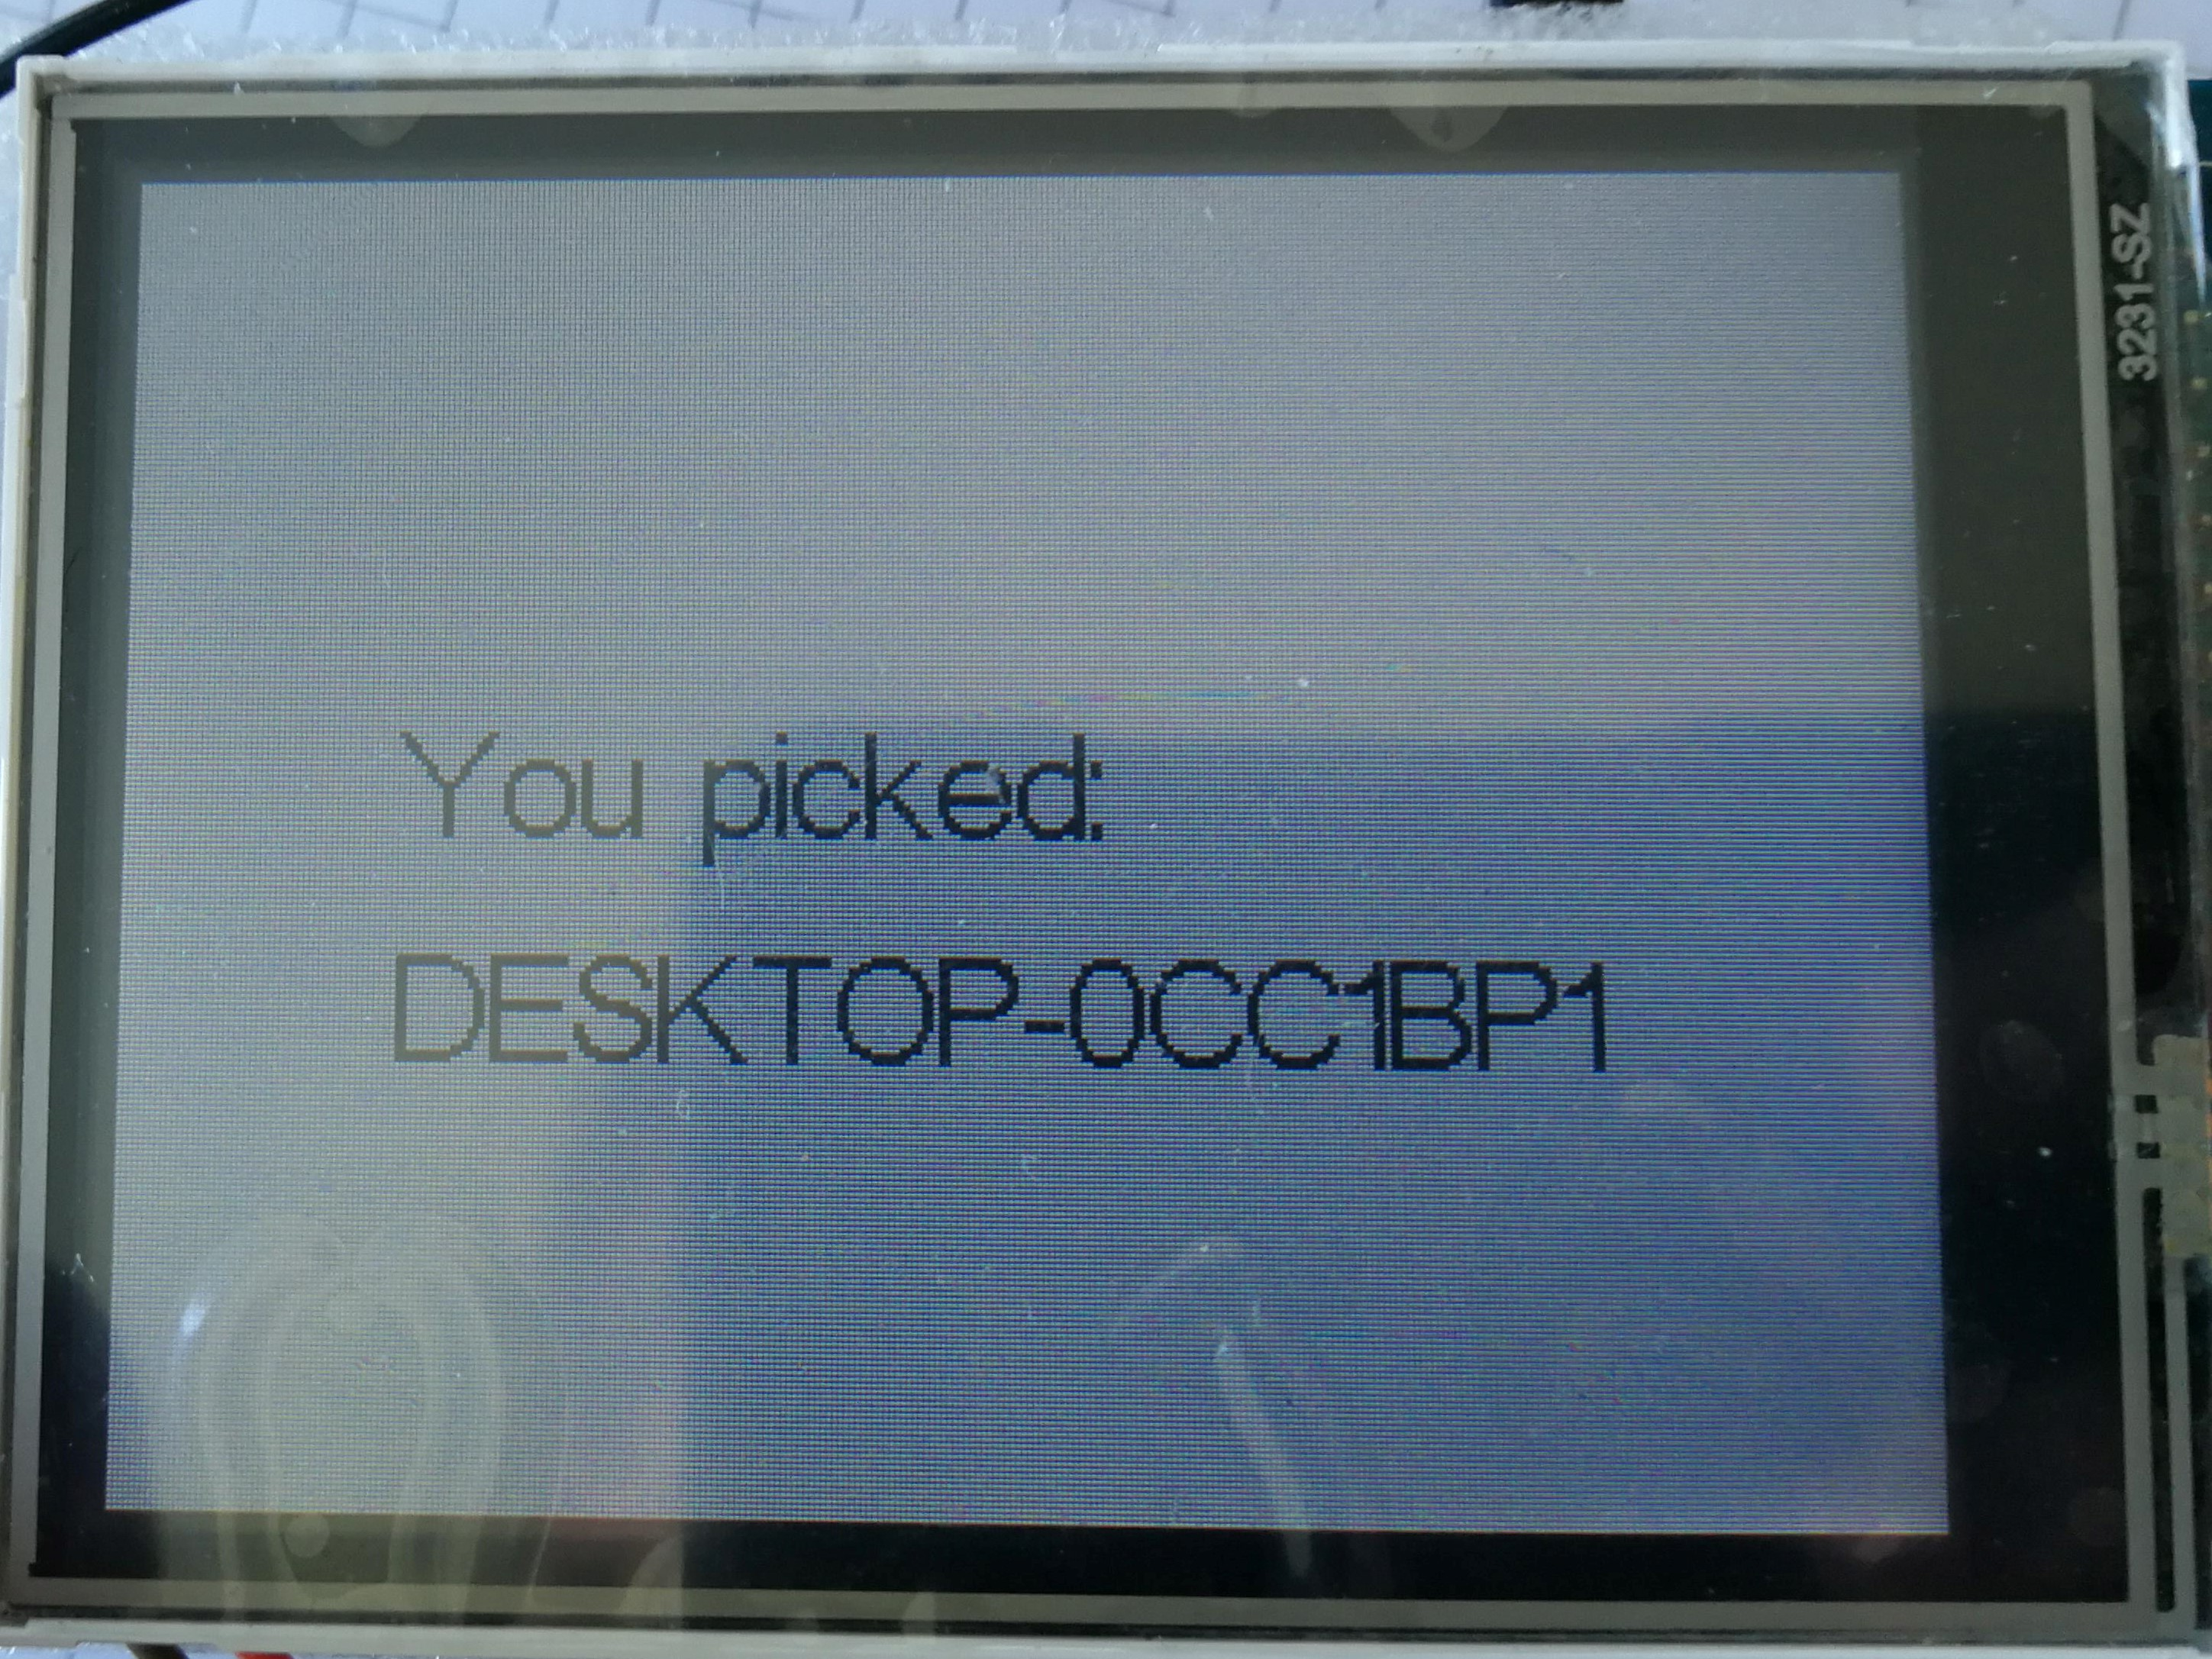
\includegraphics[width = 300 pt]{Img/pick.jpg}
	\caption{Valg af enhed}
	\label{fig:pick}
\end{figure}
Hvis brugeren herefter vælger funktionen "REMOVE DEVICE" fra figur \ref{fig:start}, åbnes der en liste over de godkendte Bluetooth-enheder der er gemt. Dette ses på figur \ref{fig:remove}. Hvis der på forhånd ikke er nogle gemte godkendte Bluetooth-enheder og listen dermed er tom, så vil displayet også være tomt, som vist på figur \ref{fig:noDevices}. 
\begin{figure}[H]
	\centering
	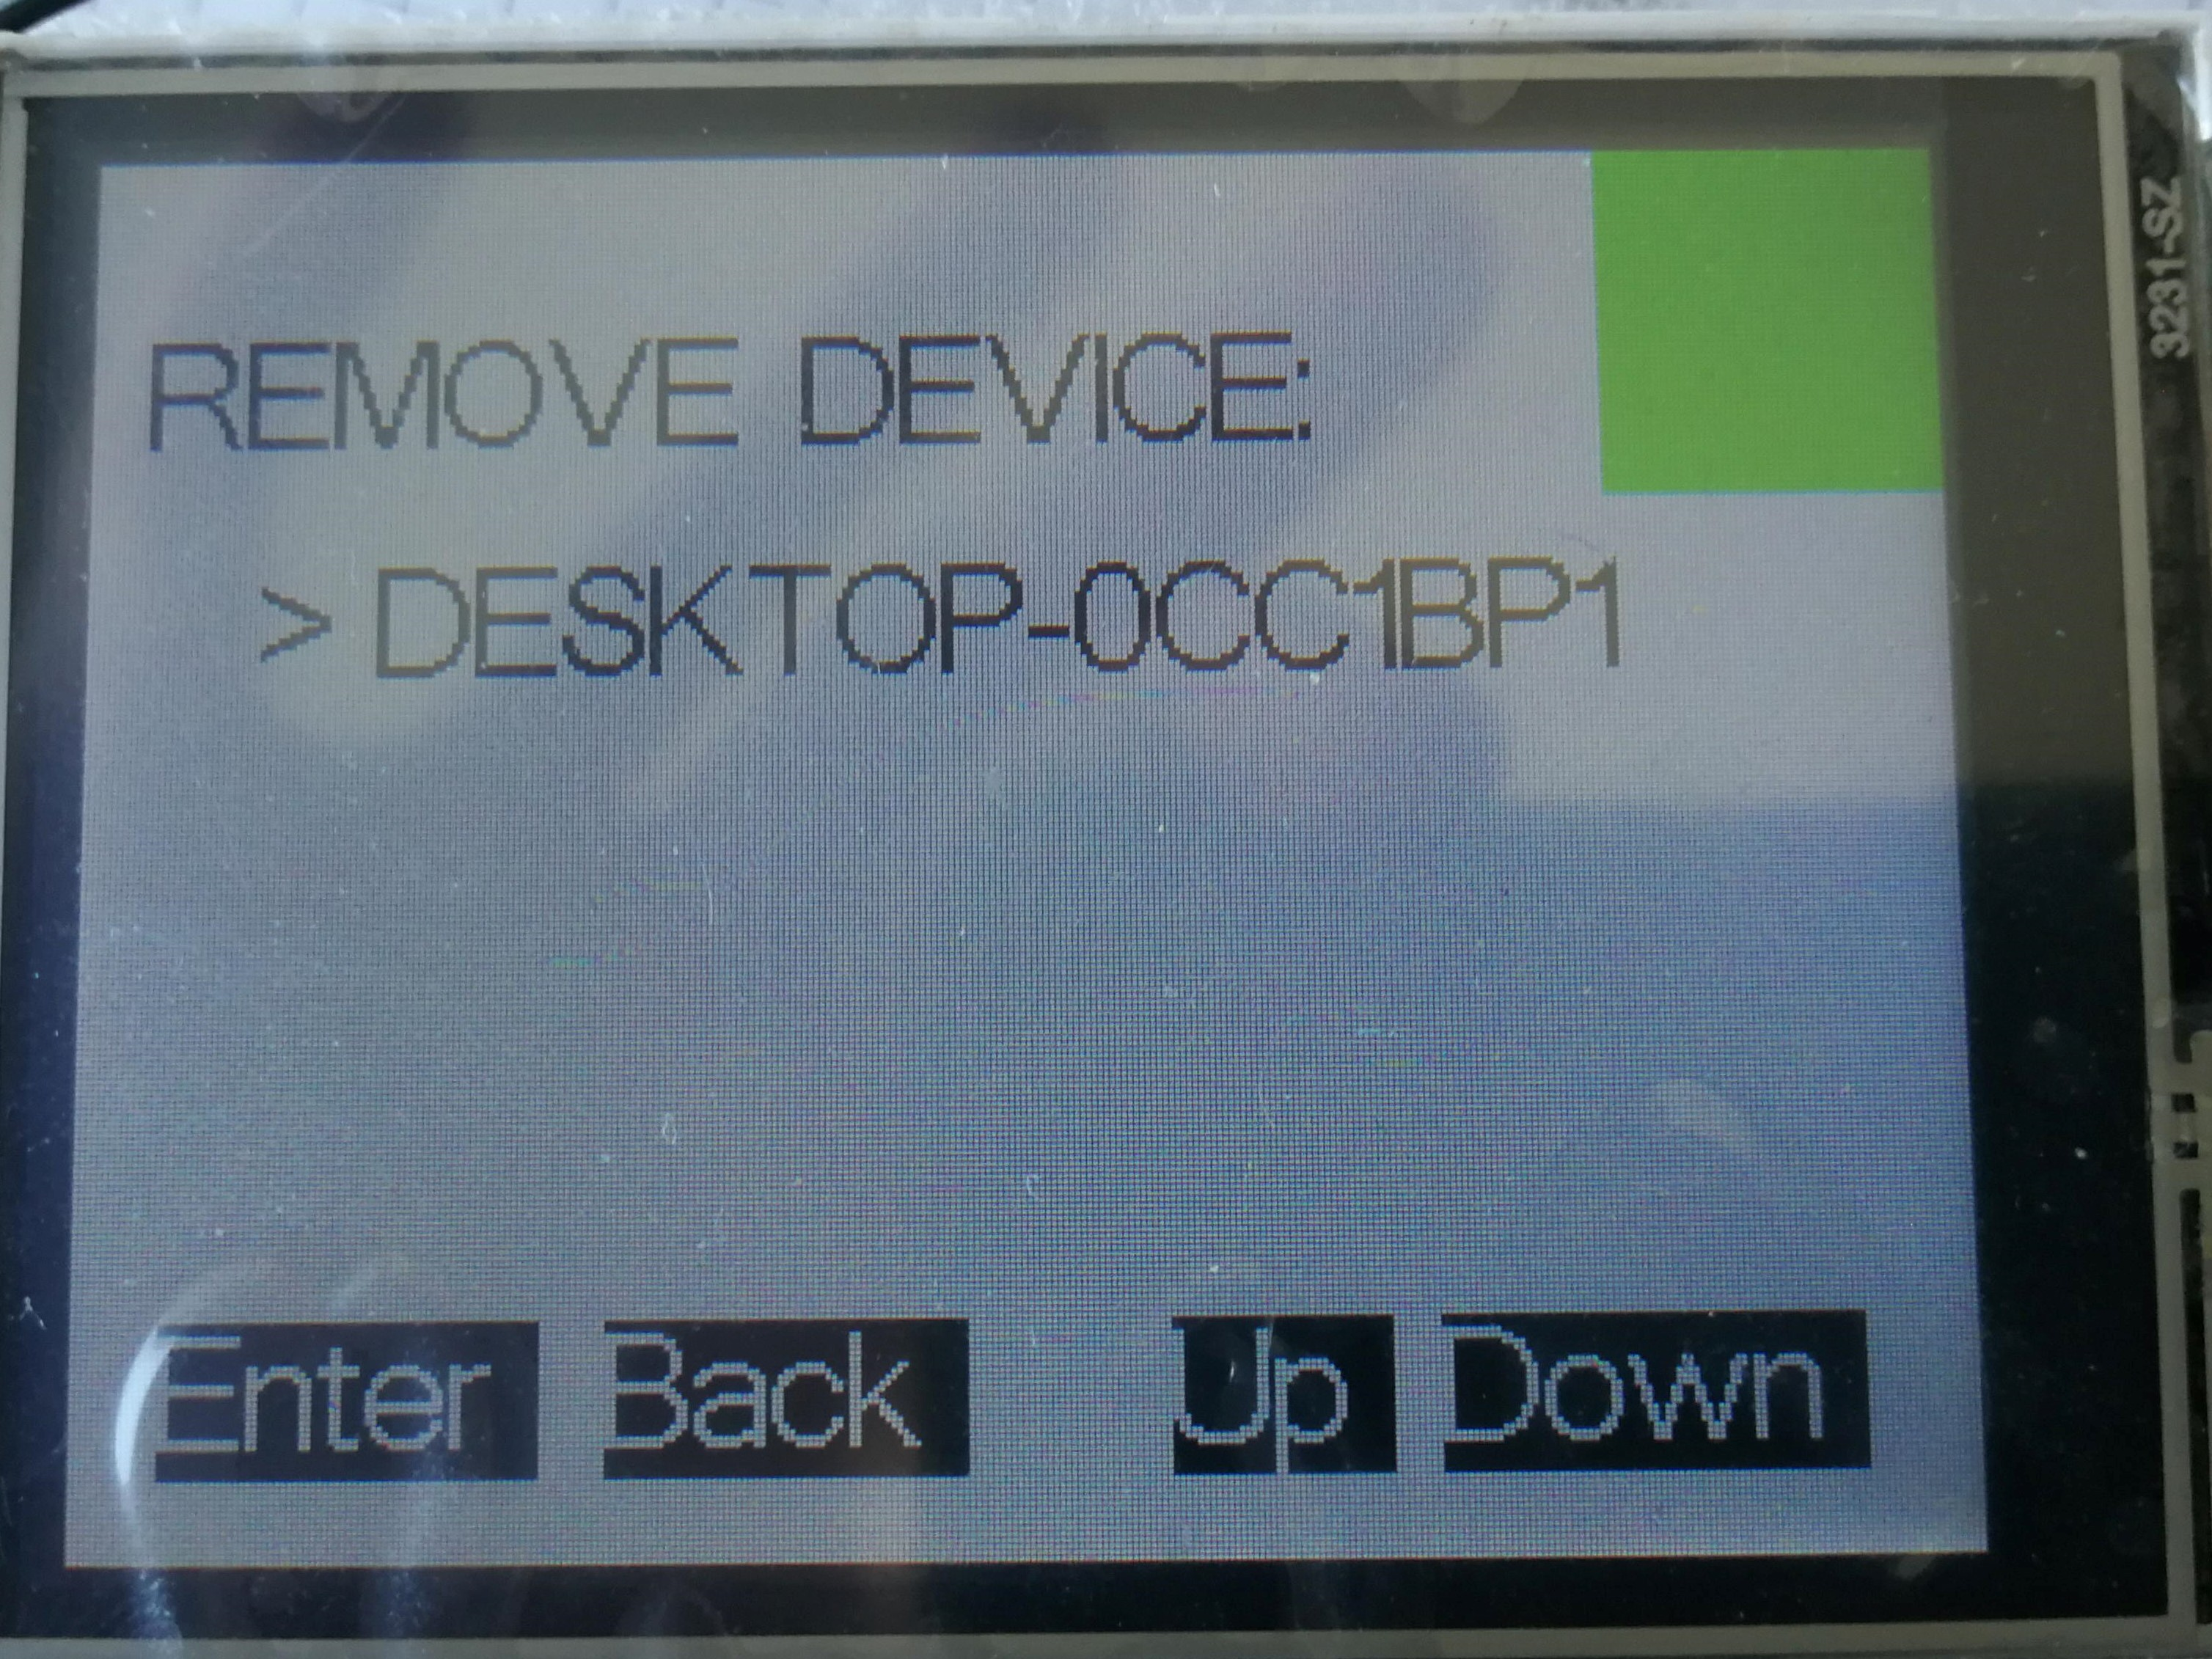
\includegraphics[width = 300 pt]{Img/remove.jpg}
	\caption{Fjern en enhed}
	\label{fig:remove}
\end{figure}
\begin{figure}[H]
	\centering
	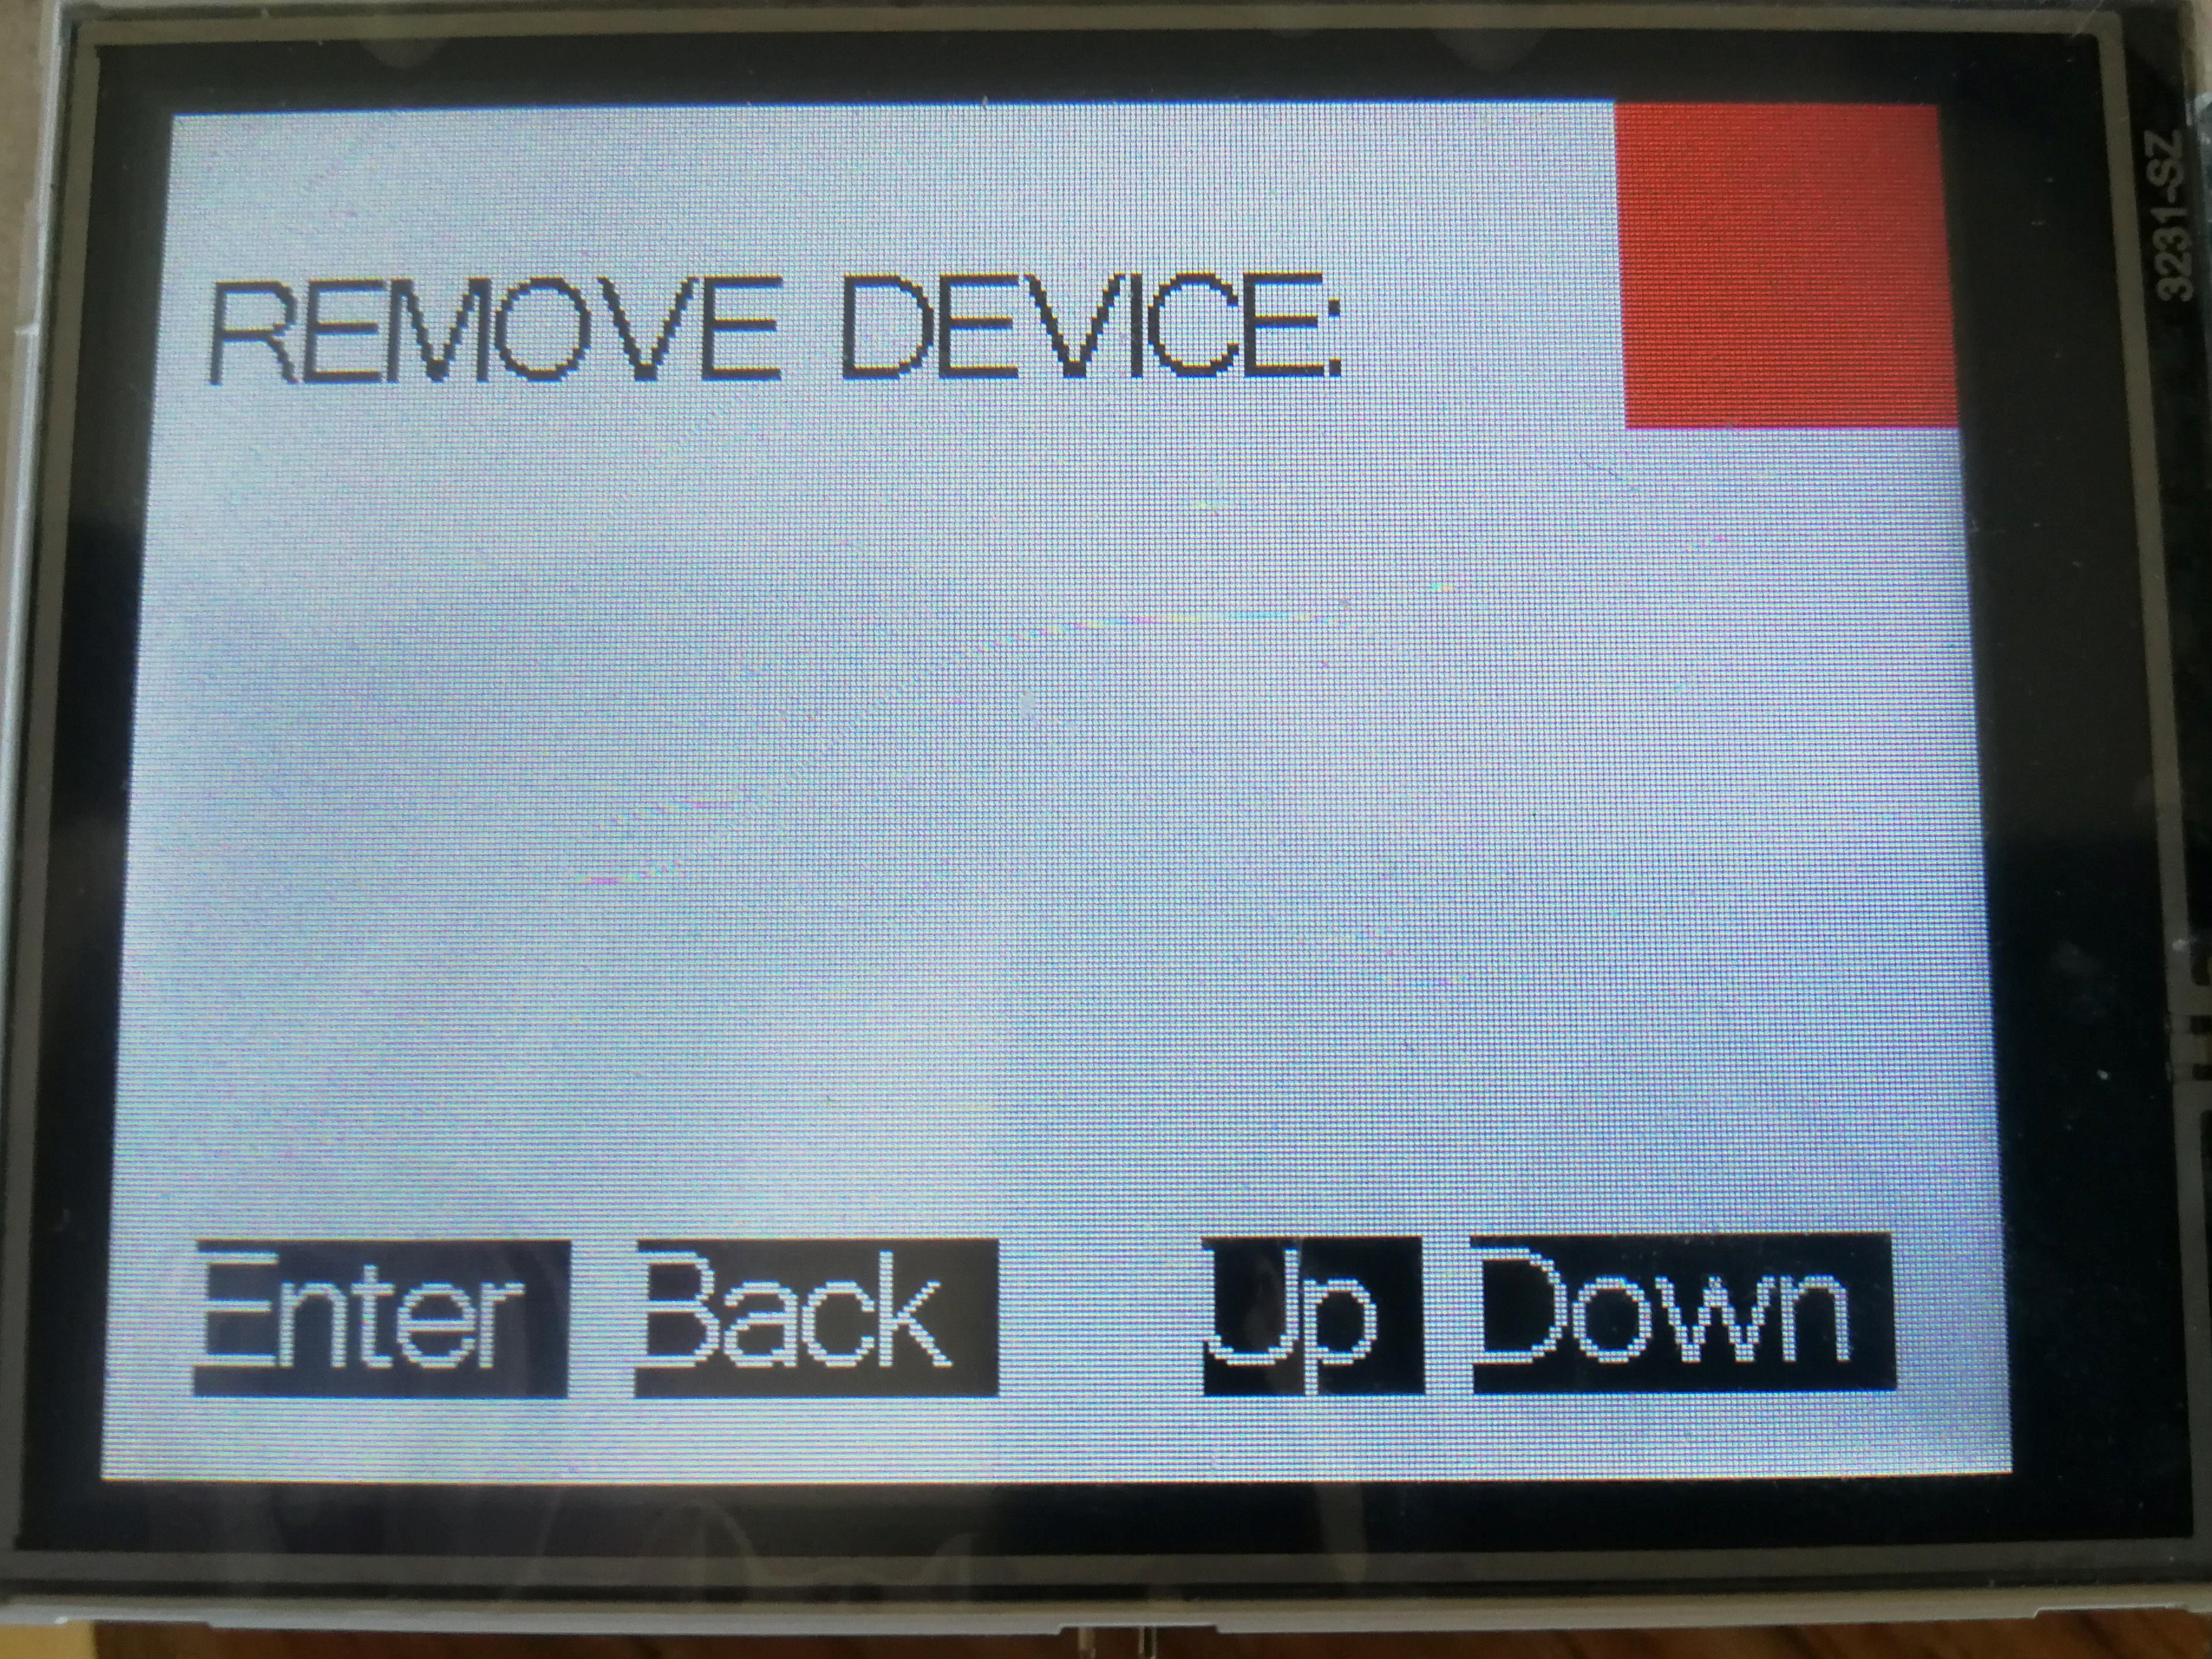
\includegraphics[width = 300 pt]{Img/noDevice.jpg}
	\caption{Ingen enehder}
	\label{fig:noDevices}
\end{figure}
Såfremt der er godkendte Bluetooth-enheder på listen, kan brugeren vælge at slette en bestemt enhed. Dette sker ved at trykke "Enter" ved enheden, som vælges ved hjælp af "Up" og "Down" og indikeres af pilen. Displayet viser på figur \ref{fig:delete} en besked om hvilken enhed brugeren har valgt at slette. 
\begin{figure}[H]
	\centering
	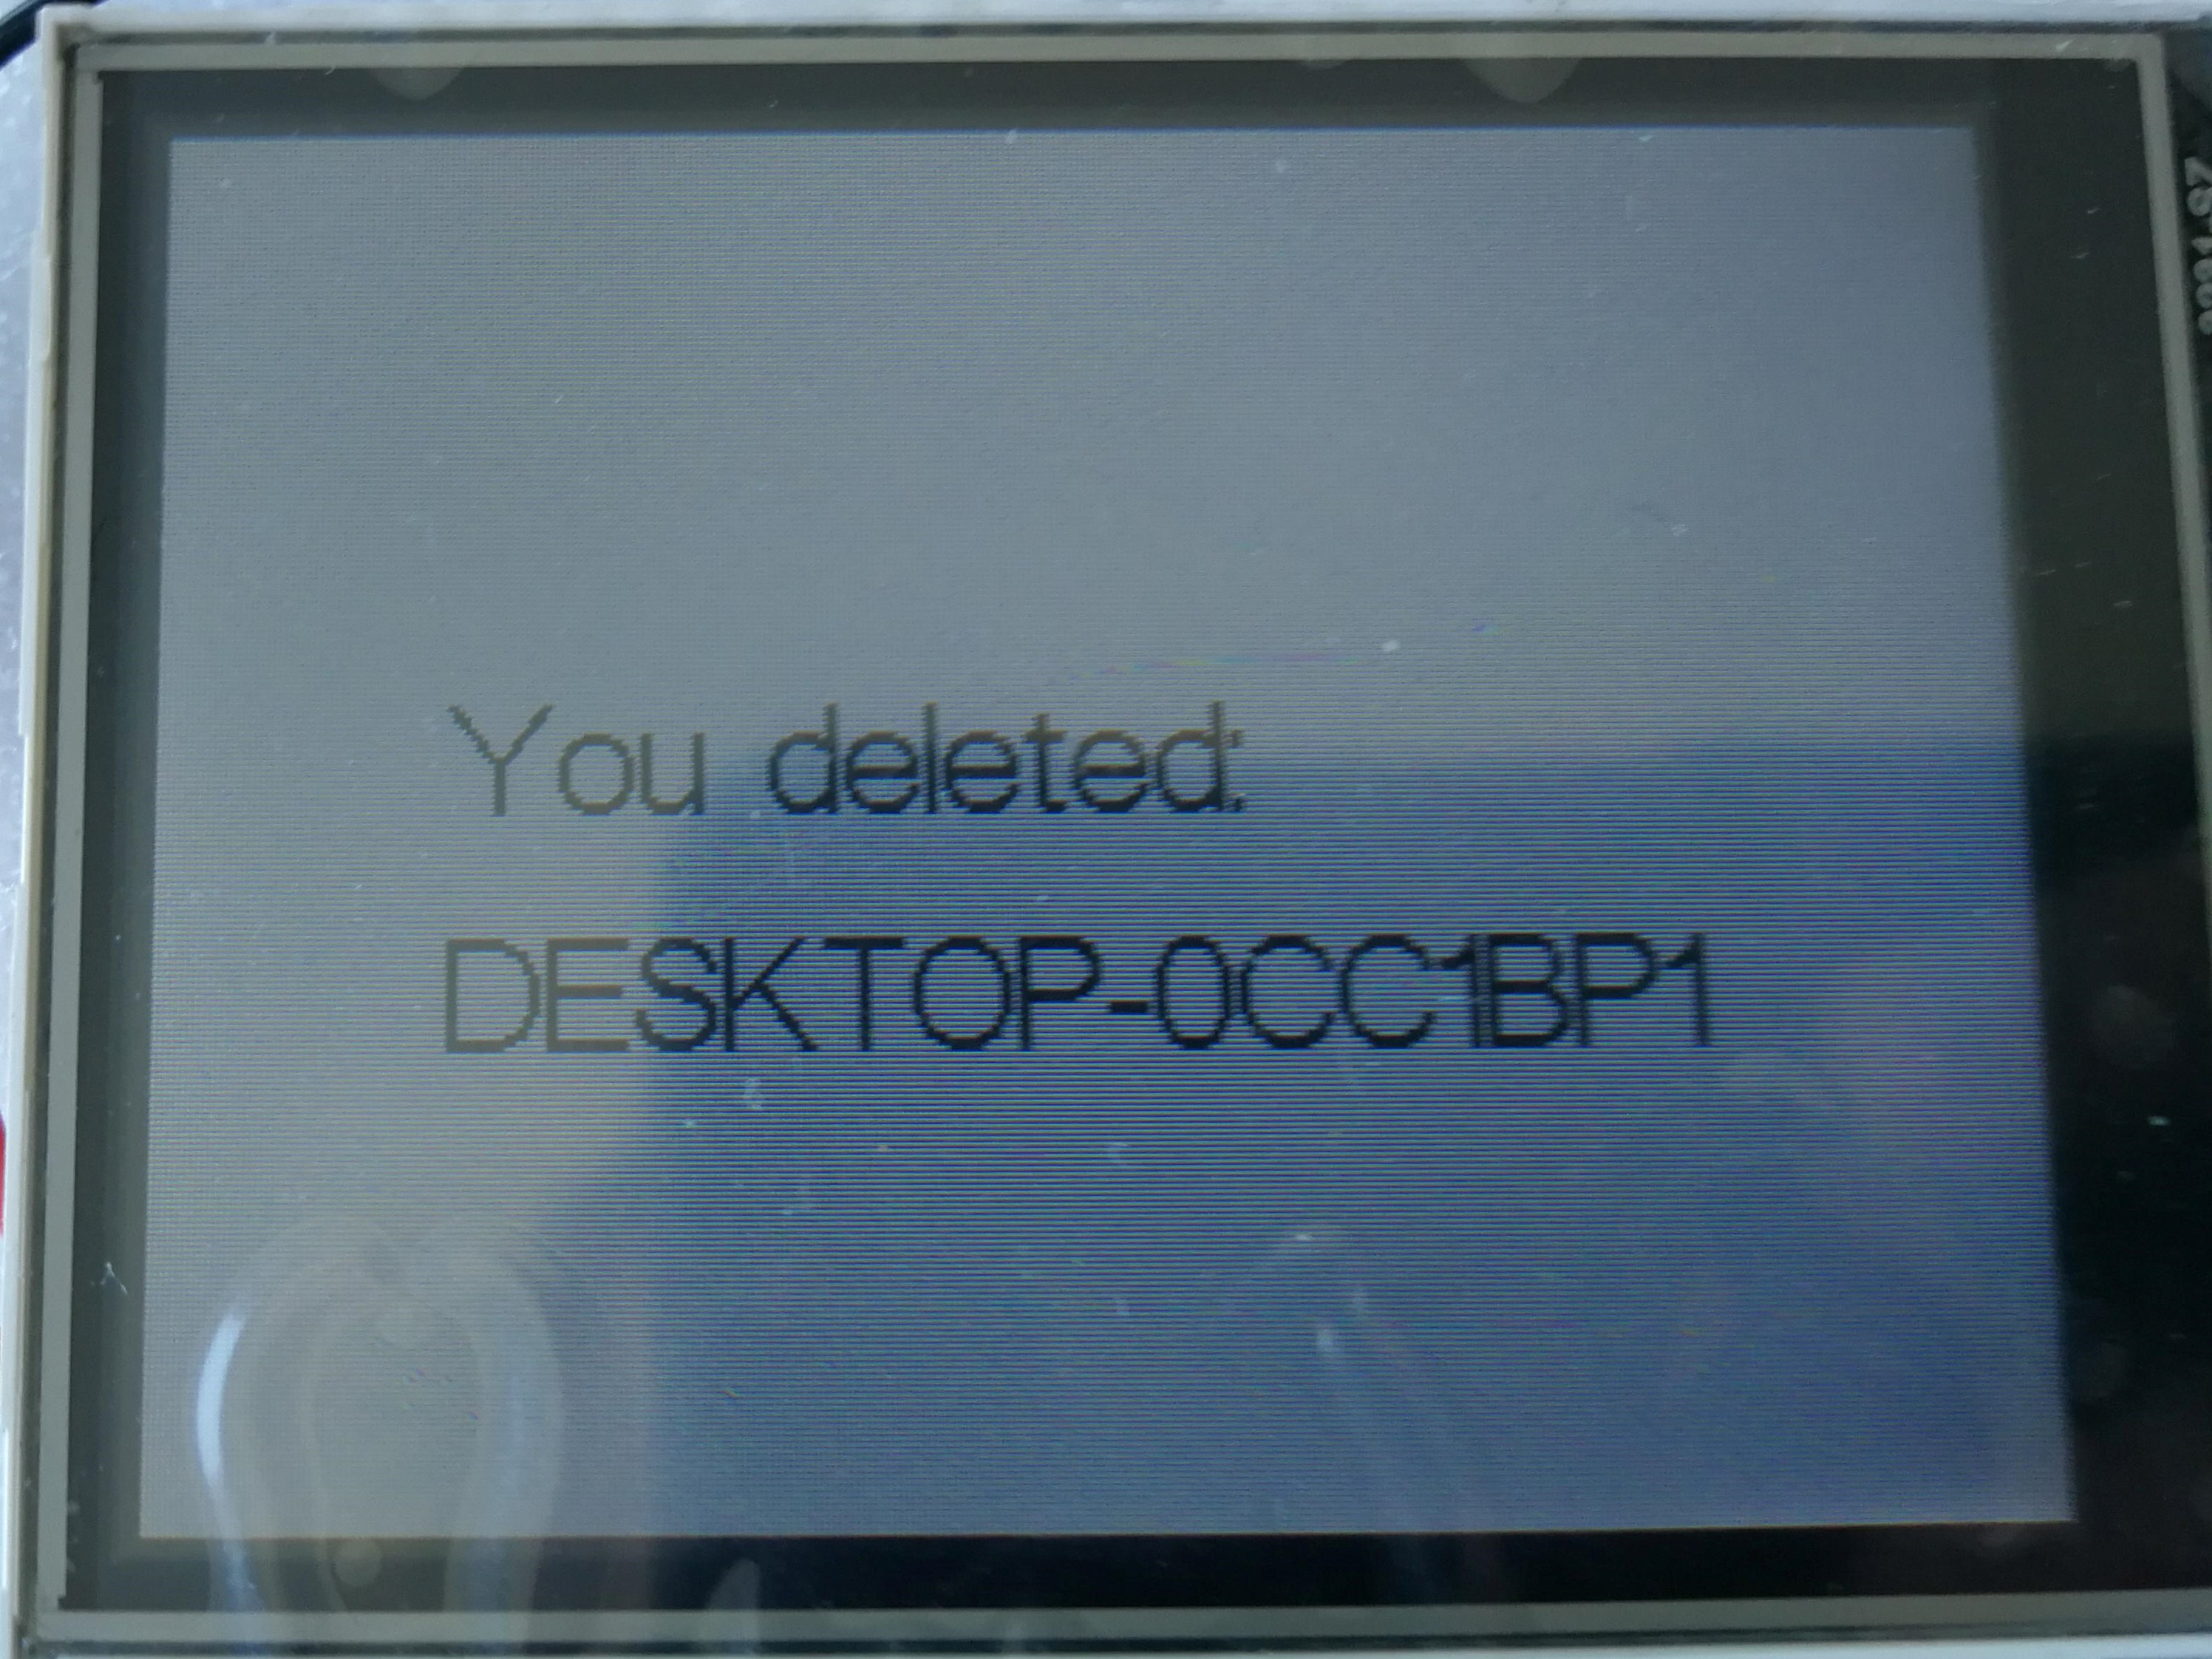
\includegraphics[width = 300 pt]{Img/delete.jpg}
	\caption{Valgt: fjernet en enhed}
	\label{fig:delete}
\end{figure}
Hvis brugeren vælger den sidste mulighed/state i hovedmenuen, "LOCK OFF", låses systemet op, teksten skifter og låsens indikator skifter farve. Dette ses på \ref{fig:lockOff}.
\begin{figure}[H]
	\centering
	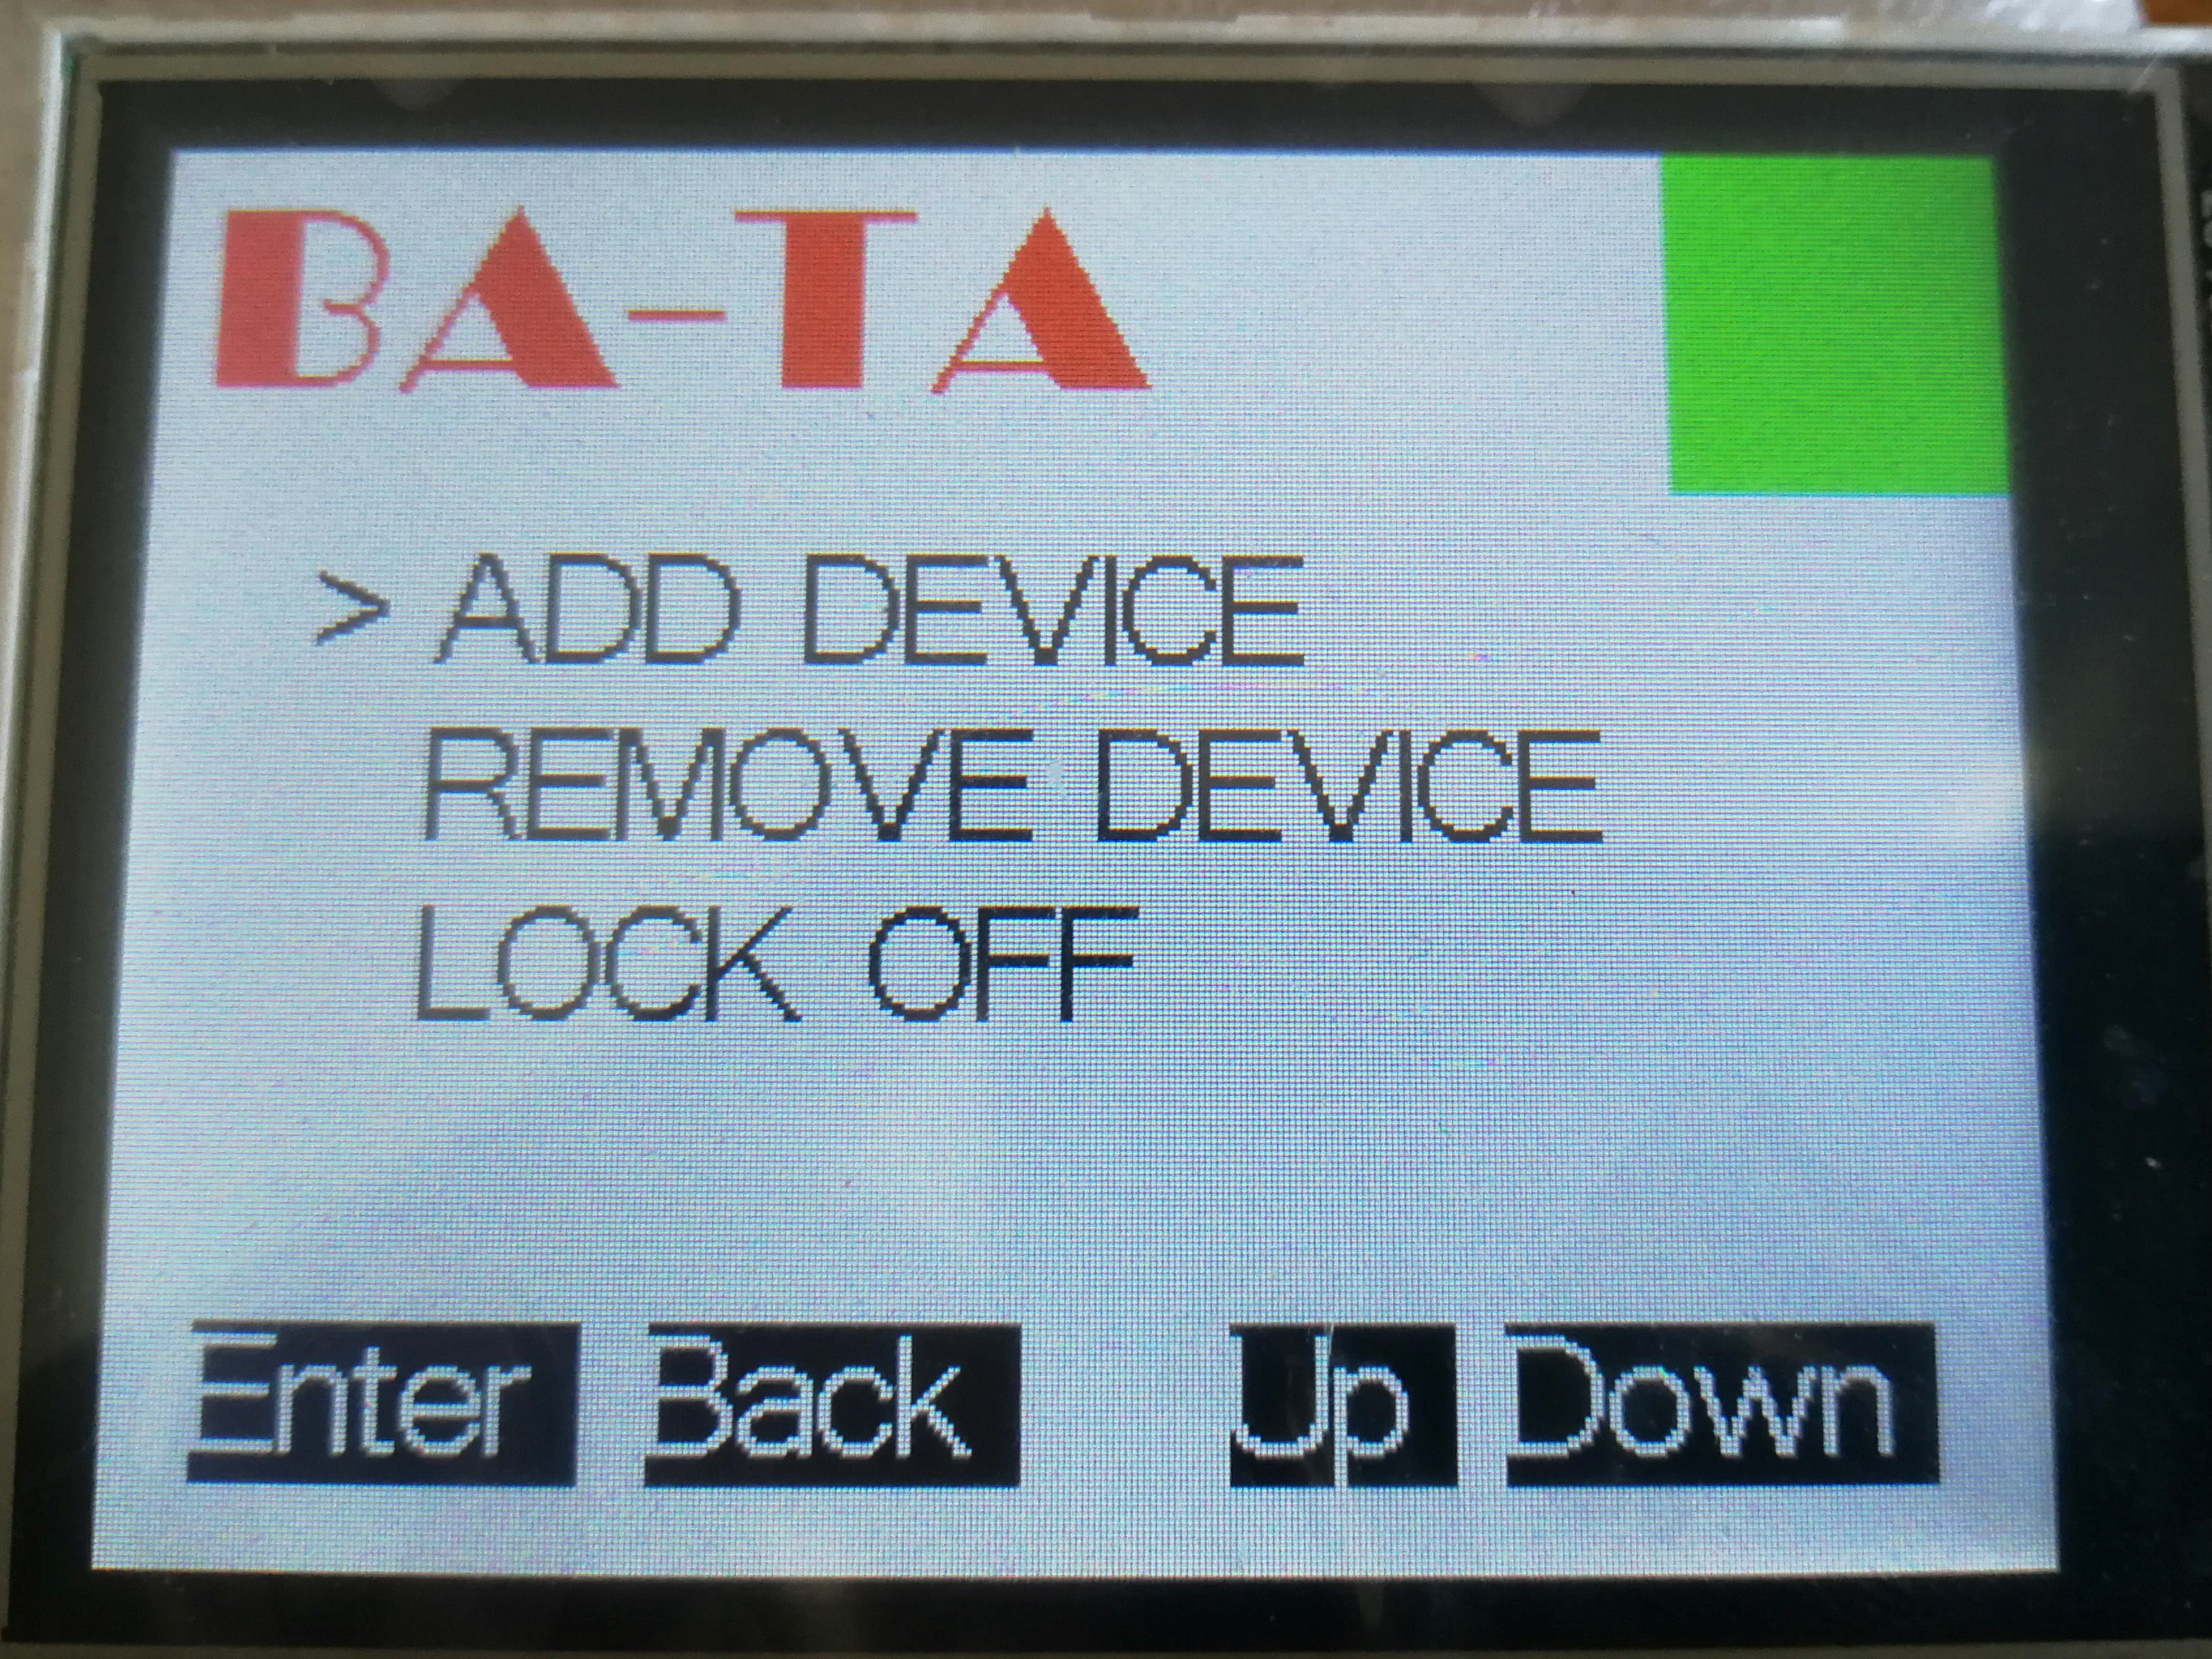
\includegraphics[width = 300 pt]{Img/lockOff.jpg}
	\caption{Låst op}
	\label{fig:lockOff}
\end{figure}
Hvis der endnu engang trykkes på den sidste state i hovedmenuen, ændres teksten, og låsen laver en "UPDATE"  hvert 5. sekund, og skifter låsen alt efter om der kan findes en Bluetooth-enhed, som også er på den godkendte liste. Dette ses på figur \ref{fig:auto}. Hvis der trykkes én gang til på sidste state, ændres låsens tilstand til at være manuelt låst.
\begin{figure}[H]
	\centering
	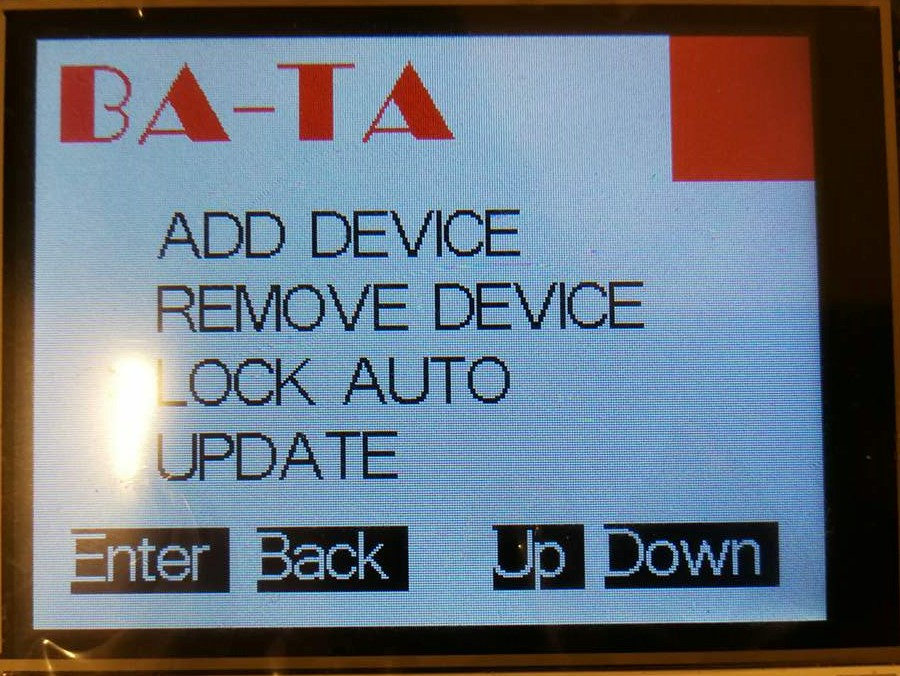
\includegraphics[width = 300 pt]{Img/auto.jpg}
	\caption{Lås Automatisk}
	\label{fig:auto}
\end{figure}

